\chapter{ Констукторский раздел}
\label{cha:design}

\section{Требования к программе}

Необходимо реализовать загружаемый модуль ядра, который будет ... TODO:
TODO: блок схема для загружаемого модуля ядра

\section{Анализируемая программа}

В качестве анализируемой программы  была выбрана программа, 
которая запускала n потоков. 
Каждый поток создавал свой собственный кольцевой односвязный список.
Далее каждый поток пробегался по всему своему односвязному списку 
и обновлял значения (заполнял рандомными значениями).
После обновления списка в конец добавлялся новый узел 
и приведенные выше операции повторялись вновь. 
На рис. \ref{fig:5} показан кольцевой односвязный список, использующийся в анализируемой программе.

\begin{figure}[ht!]
	\centering{
		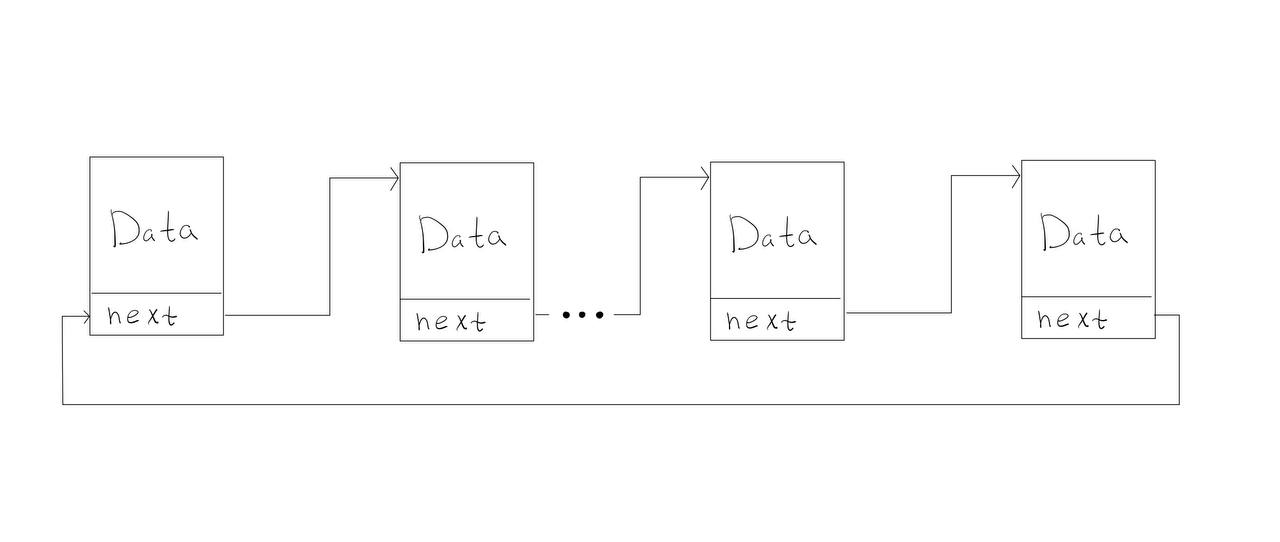
\includegraphics[width=1\textwidth]{img/5.jpeg}
		\caption{Кольцевой односвязный список}
		\label{fig:5}}
\end{figure}

На рис. \ref{fig:6} блок-схема алгоритма, который выполняет каждый поток. 

\begin{figure}[ht!]
	\centering{
		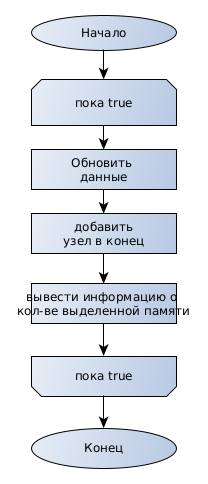
\includegraphics[width=0.4\textwidth]{img/6.png}
		\caption{Блок-схема алгоритма выполнения потока}
		\label{fig:6}}
\end{figure}



\section{Вывод}

В данном разделе было рассмотрено ...






